
\chapter{枝刈りによる探索空間の削減}
\label{chap:reduce-by-prune}
枝刈りによって探索空間を削減する.
本稿では,直径の下界を計算し,定理\ref{thm:gmg-geometric-property}
の条件\ref{gmg-geom-b}を満足するか求めることで実現する.

\section{直径の下界の計算}
\label{sect:diameter-lower-bound}
直径の下界を計算する方法を与える.まず,次のグラフを定義する.
\begin{definition}
  探索途中のグラフ$G$と候補辺番号$i$に対するオペレータの適応を行う前とする.
  この状態について,グラフ$G$に候補辺番号$i$以降のすべての辺($E'=\{e_j\}_{j>i}$)
  を追加したグラフ$G+E'$を\textbf{最大グラフ}と定義する.
  このとき,最大グラフのもとになったグラフ$G$を\textbf{最小グラフ}と呼ぶ.
\end{definition}
\begin{example}
  図\ref{fig:min-max-graph}に最小グラフと最大グラフの例を示す.
  最小グラフの破線部分はオペレータ適応の判定が行われていない候補辺を表す.
  最大グラフは,最小グラフのオペレータ適応未決定の辺をすべて追加したグラフと
  なっている.
\end{example}
\begin{figure}
  \centering
  \subfloat[最小グラフ]{
    \includegraphics[width=.4\linewidth]
                    {min-graph-example.pdf}
  }\hfill
  \subfloat[最大グラフ]{
    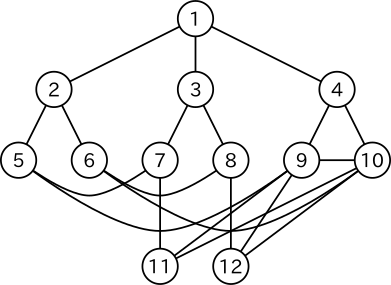
\includegraphics[width=.4\linewidth]
                    {max-graph-example.pdf}
  }
  \caption{最小グラフと最大グラフの例}
  \label{fig:min-max-graph}
\end{figure}
直径の下界は,最大グラフの直径を計算すればよい.もし直径の下界が
定理\ref{thm:gmg-geometric-property}の条件\ref{gmg-geom-b}を
満たさない場合,それ以降どのように辺を追加しても条件を満たさないので,
その場で探索を打ちきることができる.
この事実を応用して,一般化ムーアグラフの探索に直径の条件を考慮した
枝刈りを与える.探索で用いる状態は,最小グラフと最大グラフと候補辺の番号の
三つ組である.

次に,追加オペレータと無追加オペレータを新たに定めた状態に適応する.
追加オペレータは,最小グラフ$G_{\min}$と最大グラフ$G_{\max}$と候補辺番号$i$に
対して,最小グラフ$G'_{\min}=G_{\min}+e_i$と最大グラフ$G'_{\max}=G_{\max}$と
次の候補辺番号$i+1$を返す.また,無追加オペレータは,最小グラフ$G_{\min}$と
最大グラフ$G_{\max}$と候補辺番号$i$に対して,最小グラフ$G'_{\min}=G_{\min}$と
最大グラフ$G'_{\max}=G_{\max}-e_i$と次の候補辺番号$i+1$を返す.
さらに,系\ref{coll:basic-noadd-operator}で示した無追加オペレータの適応条件は
次のようになる.
\begin{collary-without-proof}
  \label{coll:minmax-noadd-operator}
  無追加オペレータについて,与えられた最小グラフを$G_{\min}$,最大グラフを
  $G_{\max}$,候補辺番号を$i$,対象の辺を$e_i=\{v,w\}$とし,
  適応後の最小グラフを$G'_{\min}$,最大グラフを$G'_{\max}$とする.
  $i$以降の辺$\{e_j\}_{j>i}$の選び方次第で
  $G_{\min}'+E\,(E\subset \{e_j\}_{j>i})$が一般化ムーアグラフとなる見込み
  があることは,次の二条件を満たすことである.
  \begin{enumerate}
  \item 次数条件$\cdots$ $\text{Exit}(x)=i$なる$x\in e_i$について,
    $d_{G'_{\min}}(x)=k$.
  \item 直径条件$\cdots$ $G'_{\max}$の直径が定理\ref{thm:gmg-geometric-property}で
    示された直径以下である.
  \end{enumerate}
\end{collary-without-proof}

最後に,枝刈りを適応した探索の手続きをアルゴリズム\ref{algo:minmax-algorithm}
に示す.これは,アルゴリズム\ref{algo:basic-algorithm}を書き換えるものである.
\begin{algorithm}[H]
  \caption{最大グラフを用いた一般化ムーアグラフの探索アルゴリズム}
  \label{algo:minmax-algorithm}
  \begin{algorithmic}[1]
    \Require $n,k$
    \Ensure $M(n,k)\:$(見つからない場合,$\varnothing$を返す)
    \Procedure{FindGeneralizedMooreGraph}{}
    \State $G_{I\min}\gets\text{初期グラフ}$
    \State $\{e_i\}_{i\in\mathbb{N}}^M\gets G_{I\min}\text{の候補辺}$
    \State $G_{I\max}\gets G_{I\min}+\{e_i\}$
    \Comment 初期グラフに対する最大グラフ
    \State $Stack\gets((G_{I\min},G_{I\max},1))$
    \While{$|Stack|>0$}
    \State $G_{\min},G_{\max},i\gets pop(Stack)$
    \If{$i>M$かつ
      $G_{\min}$が正則で定理\ref{thm:gmg-geometric-property}を満たす}
    \State \textbf{return} $G_{\min}$
    \EndIf
    \ForAll{$operator\in\{\text{無追加オペレータ},\text{追加オペレータ}\}$}
    \If{$operator$が$G_{\min},G_{\max},i$に適応できる}
    \Comment 系\ref{coll:basic-add-operator}と系\ref{coll:minmax-noadd-operator}
    \State $push(Stack,operator(G_{\min},G_{\max},i))$
    \EndIf
    \EndFor
    \EndWhile
    \State \textbf{return} $\varnothing$
    \EndProcedure
  \end{algorithmic}
\end{algorithm}

\section{頂点間距離の高速な更新法}
\label{sect:fast-distance-update}
\ref{sect:apply-to-gmg}節と\ref{sect:diameter-lower-bound}節にて,
グラフが一般化ムーアグラフになり得るかを判定するには,追加する辺に接続する
二つの頂点間距離と,直径の下界を求める必要があることを述べた.
本節では,これらの値を高速に計算するため,辺の挿入と削除に対して頂点間距離を
更新するアルゴリズムを与える.この方法の導入により,
探索空間の削減にはつながらないが,計算量が削減され実行時間の短縮が期待できる.

グラフ$G=(V,E),V=\{1,\ldots n\}$のすべての頂点の組$\{s,t\}$の距離$d(s,t)$と
距離が$d(s,t)$となる最短経路の数$\sigma(s,t)$が与えられているとする.
便宜上,$s=t$の場合はそれぞれ$d(s,s)=0,\,\sigma(s,s)=1$とする.
まず,$d(s,t)$と$\sigma(s,t)$について,追加と削除に共通するいくつかの
補題を示す.
\begin{lemma-without-proof}[Brandes\cite{Brandes2001}]
  \label{lemma:distance-1}
  $G=(V,E)$の異なる二頂点$s,t\in V$に対して,$s$から$t$への最短経路
  $G_{st}=(V_{st},E_{st})$が$v\in V$を含む,すなわち$v\in V_{st}$であるための
  必要十分条件は
  \[ d(s,t)=d(s,v)+d(v,t) \]
  が成り立つことである.
\end{lemma-without-proof}
\begin{lemma-without-proof}[難波ら\cite{Nanba2016}]
  \label{lemma:distance-2}
  $G=(V,E)$の異なる二頂点$s,t\in V$と辺$\{v,w\}\in E$を考える.
  $s$から$t$への最短経路$G_{st}=(V_{st},E_{st})$が辺$\{v,w\}$を含む,
  すなわち$\{v,w\}\in E_{st}$が成り立つための必要十分条件は
  \[ d(s,t)=d(s,v)+d(w,t)+1 \]
  が成り立つことである.ただし,$d(s,v)\leq d(s,w)$とする.
\end{lemma-without-proof}
\begin{lemma-without-proof}[Brandes\cite{Brandes2001}]
  \label{lemma:path-num-1}
  $G=(V,E)$の異なる二頂点$s,t\in V$に対して,$s$から$t$への最短経路の中で
  $v$を通るものの個数$\sigma_v(s,t)$は次式で与えられる.
  \[ \sigma_v(s,t)=\begin{aligned}\begin{cases}
    \sigma(s,v)\sigma(v,t) & d(s,t)=d(s,v)+d(v,t)\text{のとき} \\
    0 & \text{それ以外のとき}
  \end{cases}\end{aligned} \]
\end{lemma-without-proof}
\begin{lemma-without-proof}[難波ら\cite{Nanba2016}]
  \label{lemma:path-num-2}
  $G=(V,E)$の異なる二頂点$s,t\in V$に対して,$s$から$t$への最短経路の中で
  辺$\{v,w\}$を通るものの個数$\sigma_{vw}(s,t)$は次式で与えられる.
  \[ \sigma_{vw}(s,t)=\begin{aligned}\begin{cases}
    \sigma(s,v)\sigma(w,t) & d(s,t)=d(s,v)+d(w,t)+1\text{のとき} \\
    0 & \text{それ以外のとき}
  \end{cases}\end{aligned} \]
  ただし,$d(s,v)\leq d(s,w)$とする.
\end{lemma-without-proof}

次の補題は,ある二頂点間の最短経路の個数と,その経路に含まれる
短い最短経路の個数との関係を示す.
\begin{lemma}
  \label{lemma:number-of-paths}
  $G=(V,E)$の異なる二頂点$s,t\in V$について,$v$を$d(s,t)=d(s,v)+d(v,t)$
  である頂点(ただし$v\neq s,t$)とすると,次が成り立つ.
  \begin{equation}
    \label{eq:number-of-paths}
    \sigma(s,t)=\frac{\sum_{v}\sigma(s,v)\sigma(v,t)}{d(s,t)-1}
  \end{equation}
\end{lemma}
\begin{proof}
  $s$と$t$の間の一般的な経路を図\ref{fig:proof-number-of-paths}に示す.
  \begin{figure}
    \centering
    \def\svgwidth{.5\columnwidth}
    \input{proof-number-of-paths.pdf_tex}
    \caption{$s$と$t$の一般的な最短経路}
    \label{fig:proof-number-of-paths}
  \end{figure}
  $s$からの距離が一定の頂点を並べて,一つの層とする.$d(s,v)=k$なる頂点
  $v$の集合を,第$k$層と定義し,$L_k$と表す.
  $L_k$に属する頂点の数を$n_k$,$L_k$に属する$l$番目の頂点を$v_{kl}$と表す.
  ここで,第$k$層に属する頂点$v$は,隣接する層(第$k-1$層と第$k+1$層)
  以外の層に属する頂点$w$と隣接しないことに注意する.
  もしそのような頂点が存在すると,最短経路長が変化する.
  式\ref{eq:number-of-paths}の両辺に$d(s,t)-1$を掛けて,
  次の式\ref{eq:number-of-paths1}を得る.
  \begin{equation}
    \sigma(s,t)(d(s,t)-1)=\sum_{v}\sigma(s,v)\sigma(v,t)
    \label{eq:number-of-paths1}
  \end{equation}
  式\ref{eq:number-of-paths1}の右辺を,
  図\ref{fig:proof-number-of-paths}にならって表すと,
  \begin{equation}
    \sum_{v}\sigma(s,v)\sigma(v,t)=
    \sum_{k=1}^m\sum_{l=1}^{n_k}\sigma(s,v_{kl})\sigma(v_{kl},t)
    \label{eq:number-of-paths2}
  \end{equation}
  が得られる.ここで,二つの頂点$v$と$w$について,次の隣接を表す記号$a$を
  導入する.
  \begin{align*}
    a(v,w)=
    \begin{cases}
      1 & vとwが隣接しているとき \\
      0 & vとwが隣接していないとき
    \end{cases}
  \end{align*}
  各々の$\sigma(s,v_{kl})\sigma(v_{kl},t)$について議論する.
  $a$の定義を用いて式を変形すると,
  \begin{align}
    &\sigma(s,v_{kl})\sigma(v_{kl},t)\nonumber\\
    =&\left(\sum_{v'\in L_{k-1}}\sigma(s,v')a(v',v_{kl})\right)
    \left(\sum_{v'\in L_{k+1}}\sigma(v_{kl},v')a(v',t)\right)
    \nonumber\\
    =&\left(\sum_{v''\in L_{k-2}}\sum_{v'\in L_{k-1}}
    \sigma(s,v'')a(v'',v')a(v',v_{kl})\right)
    \left(\sum_{v'\in L_{k+1}}\sum_{v''\in L_{k+2}}
    a(v_{kl},v')a(v',v'')\sigma(v'',t)\right)
    \nonumber\\
    &\vdots\nonumber\\
    =&\left(\sum_{(v_1,\ldots,v_{k-1})\in L_1\times\cdots\times L_{k-1}}
    a(s,v_1)\cdots a(v_{k-1},v_{kl})\right)
    \left(\sum_{(v_{k+1},\ldots,v_m)\in L_{k+1}\times\cdots\times L_m}
    a(v_{kl},v_{k+1})\cdots a(v_m,v_t)\right)\nonumber\\
    =&\sum_{
      (v_1,\ldots,v_{k-1},v_{k+1},\ldots,v_m)\in
      L_1\times\cdots\times L_{k-1}\times L_{k+1}\times\cdots\times L_m
    }
    a(s,v_1)\cdots a(v_{k-1},v_{kl})a(v_{kl},v_{k+1})\cdots a(v_m,t)
    \label{eq:number-of-paths3}
  \end{align}
  が得られる.式\ref{eq:number-of-paths3}を式\ref{eq:number-of-paths2}に
  代入すると,
  \begin{align}
    &\sum_{k=1}^m\sum_{l=1}^{n_k}\sigma(s,v_{kl})\sigma(v_{kl},t)\nonumber\\
    =&\sum_{k=1}^m\sum_{l=1}^{n_k}\sum_{
      (v_1,\ldots,v_{k-1},v_{k+1},\ldots,v_m)\in
      L_1\times\cdots\times L_{k-1}\times L_{k+1}\times\cdots\times L_m
    }
    a(s,v_1)\cdots a(v_{k-1},v_{kl})a(v_{kl},v_{k+1})\cdots a(v_m,t)\nonumber\\
    =&\sum_{k=1}^m\sum_{(v_1,\ldots,v_m)\in L_1\times\cdots\times L_m}
    a(s,v_1)\cdots a(v_m,t)\nonumber\\
    =&m\left(\sum_{(v_1,\ldots,v_m)\in L_1\times\cdots\times L_m}
    a(s,v_1)\cdots a(v_m,t)\right)
    \label{eq:number-of-paths4}
  \end{align}
  と変形できる.式\ref{eq:number-of-paths4}の総和の対象が$1$となるのは,
  $a(s,v_1),\ldots,a(v_m,t)$のすべてが$1$のとき,
  すなわち,$s$と$v_1$,$v_1$と$v_2$,$\ldots$,$v_m$と$t$がすべて隣接している
  とき,すなわち,$s$と$t$の最短経路となっているときである.
  従って,総和の値は$s$と$t$の最短経路の数と一致し,
  式\ref{eq:number-of-paths4}は$\sigma(s,t)(d(s,t)-1)$と等しい.
  従って,補題が成り立つ.
\end{proof}

\subsection*{辺の挿入に対する頂点間距離の更新}
$G$に辺$e=\{\alpha,\beta\}\notin E(G)$を挿入したた後の頂点間距離$d'(s,t)$と
最短経路数$\sigma'(s,t)$を求める.
ここでは,難波ら\cite{Nanba2016}が提案した方法に関する重要な定理と
アルゴリズムを示す.
\begin{theorem-without-proof}[難波ら\cite{Nanba2016}]
  \label{thm:update-distance-on-insert}
  グラフ$G=(V,E)$から辺$\{\alpha,\beta\}\notin E$を追加した後の
  頂点間距離$d'(s,t)$と最短経路数$\sigma'(s,t)$について,次が成り立つ.
  ただし,$d(s,\alpha)\leq d(s,\beta)$とする.
  \begin{enumerate}
  \item $d(s,\alpha)<d(s,\beta)$かつ$d(s,t)>d(s,\alpha)+d(\beta,t)+1$ならば,
    次が成り立つ.
    \[ d'(s,t)=d(s,\alpha)+d(\beta,t)+1,\:
    \sigma'(s,t)=\sigma(s,\alpha)\sigma(\beta,t) \]
  \item $d(s,\alpha)<d(s,\beta)$かつ$d(s,t)=d(s,\alpha)+d(\beta,t)+1$ならば,
    次が成り立つ.
    \[ d'(s,t)=d(s,t),\:
    \sigma'(s,t)=\sigma(s,t)+\sigma(s,\alpha)\sigma(\beta,t) \]
  \item $d(s,\alpha)=d(s,\beta)$または$d(s,t)<d(s,\alpha)+d(\beta,t)+1$ならば,
    次が成り立つ.
    \[ d'(s,t)=d(s,t),\:\sigma'(s,t)=\sigma(s,t) \]
  \end{enumerate}
\end{theorem-without-proof}

定理\ref{thm:update-distance-on-insert}を元にして,
辺の挿入に対する$d(s,t)$と$\sigma(s,t)$の更新の手順を与える.
それをアルゴリズム\ref{algo:update-distance-on-insert}に示す.
\begin{algorithm}[H]
  \caption{辺$\{\alpha,\beta\}$が追加されたときの$d'(s,t)$と$\sigma'(s,t)$の
    更新}\label{algo:update-distance-on-insert}
  \begin{algorithmic}[1]
    \Require $G=(V,E),\,d(s,t),\,\sigma(s,t)$
    \Ensure $d'(s,t),\,\sigma'(s,t)$
    \ForAll{$(s,t)\in V\times V,\,s<t$}
    \State $(\alpha,\beta)$のうち$s$に近いほうを$\alpha$とする
    \If{$d(s,\alpha)<d(s,\beta)$かつ$d(s,t)>d(s,\alpha)+d(\beta,t)+1$}
    \State $d'(s,t)\gets d(s,\alpha)+d(\beta,t)+1$
    \State $\sigma'(s,t)\gets \sigma(s,\alpha)\sigma(\beta,t)$
    \ElsIf{$d(s,\alpha)<d(s,\beta)$かつ$d(s,t)=d(s,\alpha)+d(\beta,t)+1$}
    \State $d'(s,t)\gets d(s,t)$
    \State $\sigma'(s,t)\gets \sigma(s,t)+\sigma(s,\alpha)\sigma(\beta,t)$
    \ElsIf{$d(s,\alpha)=d(s,\beta)$または$d(s,t)<d(s,\alpha)+d(\beta,t)+1$}
    \State $d'(s,t)\gets d(s,t)$
    \State $\sigma'(s,t)\gets\sigma(s,t)$
    \Else
    \EndIf
    \EndFor
  \end{algorithmic}
\end{algorithm}

\subsection*{辺の削除に対する頂点間距離の更新}
$G$から辺$e=\{\alpha,\beta\}\in E(G)$を削除した後の頂点間距離$d'(s,t)$と
最短経路数$\sigma'(s,t)$を求める.次の定理が成り立つ.
\begin{theorem}
  \label{thm:update-distance-on-delete}
  グラフ$G=(V,E)$から辺$\{\alpha,\beta\}\in E$を削除した後の
  頂点間距離$d'(s,t)$と最短経路数$\sigma'(s,t)$について,次が成り立つ.
  ただし,$d(s,\alpha)\leq d(s,\beta)$とする.
  \begin{enumerate}
  \item $\sigma_{\alpha\beta}(s,t)=0$ならば,次が成り立つ.
    \[ d'(s,t)=d(s,t),\:\sigma'(s,t)=\sigma(s,t) \]
  \item $0<\sigma_{\alpha\beta}(s,t)<\sigma(s,t)$ならば,次が成り立つ.
    \[ d'(s,t)=d(s,t),\:\sigma'(s,t)=\sigma(s,t)-\sigma_{\alpha\beta}(s,t) \]
  \item $\sigma_{\alpha\beta}(s,t)=\sigma(s,t)>0$ならば,次が成り立つ.
    \begin{equation*}
      \begin{aligned}
        d'(s,t)&=\min\{d(s,v)+d(v,t)\,|\,v\in V,\,
        \sigma(s,v)>\sigma_{\alpha\beta}(s,v),\,
        \sigma(v,t)>\sigma_{\alpha\beta}(v,t) \\
        \sigma'(s,t)&=\frac{\sum_v(\sigma'(s,v)\sigma'(v,t))}{d'(s,t)-1}\:
        (v\in V,\,v\neq s,t,\,d'(s,t)=d'(s,v)+d'(v,t))
      \end{aligned}
    \end{equation*}
  \end{enumerate}
\end{theorem}
\begin{proof}
  辺削除による更新の操作は次の三種類である.
  \begin{enumerate}
  \item 削除による影響はなく,何も行わない
  \item 削除により最短経路数を更新する
  \item 削除により頂点間距離を更新し,さらに最短経路数を再計算する
  \end{enumerate}

  一つ目の操作が実施される場合は,辺$\{\alpha,\beta\}$が$s$と$t$との
  最短経路に含まれていないときである.これは,補題\ref{lemma:path-num-2}より,
  $\sigma_{\alpha\beta}(s,t)=0$のときと言い換えられる.

  二つ目の操作が実施される場合は,
  $s$と$t$との最短経路の集合$P\neq\varnothing$と,
  $P$の中で辺$\{\alpha,\beta\}$を含む経路の集合$P'\neq\varnothing$に対して,
  $P'\subset P$のときである.
  言い換えると,補題\ref{lemma:path-num-2}より,
  $0<\sigma_{\alpha\beta}(s,t)<\sigma(s,t)$のときである.
  このとき,削除により$P'$に属する最短経路がなくなるため,
  その数($\sigma_{\alpha\beta}(s,t)$)だけ$\sigma(s,t)$から引いた値とする.

  三つ目の操作が実施される場合は,
  $s$と$t$との最短経路の集合$P\neq\varnothing$と,
  $P$の中で辺$\{\alpha,\beta\}$を含む経路の集合$P'\neq\varnothing$に対して,
  $P'=P$のときである.
  言い換えると,補題\ref{lemma:path-num-2}より,
  $\sigma_{\alpha\beta}(s,t)=\sigma(s,t)>0$のときである.
  このとき,削除により$P$に属する最短経路がすべて無効になるため,頂点間距離を
  再計算する.補題\ref{lemma:distance-1}より,
  新しい頂点間距離$d'(s,t)$を計算できる.このとき,中間の頂点$v$は
  削除による頂点間距離の更新が起こらない頂点を選ぶ.
  また,新しい最短経路数$\sigma'(s,t)$は補題\ref{lemma:number-of-paths}により
  計算できる.
\end{proof}

定理\ref{thm:update-distance-on-delete}より,一辺削除時の頂点間距離の
更新の方法が分かる.
その手順ををアルゴリズム\ref{algo:update-distance-on-delete}に示す.
\begin{algorithm}[H]
  \caption{辺$\{\alpha,\beta\}$が削除されたときの$d'(s,t)$と$\sigma'(s,t)$の
    更新}\label{algo:update-distance-on-delete}
  \begin{algorithmic}[1]
    \Require $G=(V,E),\,d(s,t),\,\sigma(s,t)$
    \Ensure $d'(s,t),\,\sigma'(s,t)$
    \State $P\gets()$
    \Comment{更新の対象となる頂点組$(s,t)$}
    \ForAll{$(s,t)\in V\times V,\,s<t$}
    \If{$\sigma_{\alpha\beta}(s,t)=0$}
    \State $d'(s,t)=d(s,t)$
    \State $\sigma'(s,t)=\sigma(s,t)$
    \ElsIf{$0<\sigma_{\alpha\beta}(s,t)<\sigma(s,t)$}
    \State $d'(s,t)=d(s,t)$
    \State $\sigma'(s,t)=\sigma(s,t)-\sigma_{\alpha\beta}(s,t)$
    \ElsIf{$\sigma_{\alpha\beta}(s,t)=\sigma(s,t)>0$}
    \Comment{頂点間距離を再計算}
    \State $d_{\min}\gets \infty$
    \ForAll{$v\in V,\,
      \sigma(s,v)>\sigma_{\alpha\beta}(s,v),\,
      \sigma(v,t)>\sigma_{\alpha\beta}(v,t)$}
    \State $d_{\min}\gets\min\left\{d_{\min},d(s,v)+d(v,t)\right\}$
    \EndFor
    \If{$d_{\min}=\infty$}
    \State $d'(s,t)\gets\infty$
    \State $\sigma'(s,t)\gets0$
    \Else
    \State $d'(s,t)\gets d_{\min}$
    \State \parbox[t]{\linewidth}{
      $P\gets(\ldots,(s_i,t_i),(s,t),(s_{i+1},t_{i+1}),\ldots)$ \\
      ただし,$d'(s_i,t_i)\leq d'(s,t)\leq d'(s_{i+1},t_{i+1}),\:$
      $\ldots,(s_i,t_i),\ldots\in P$
    }
    \EndIf
    \EndIf
    \EndFor
    \ForAll{$(s_i,t_i)\in P$}
    \Comment{最短経路数を再計算}
    \State $\sigma'\gets0$
    \ForAll{$v\in V,\:v\neq s_i,t_i,\:d'(s_i,t_i)=d'(s_i,v)+d'(v,t_i)$}
    \State $\sigma'\gets\sigma'+\sigma'(s_i,v)\sigma'(v,t_i)$
    \EndFor
    \State $\sigma'(s_i,t_i)\gets\sigma'/(d'(s_i,t_i)-1)$
    \EndFor
  \end{algorithmic}
\end{algorithm}

アルゴリズム\ref{algo:update-distance-on-delete}では,頂点間距離の
再計算の対象の組$(s,t)$を$d'(s,t)$の昇順になるようにリストに追加している.
この根拠は次の系\ref{coll:update-distance-on-delete}で与える.
\begin{collary}
  \label{coll:update-distance-on-delete}
  頂点間距離を再計算した組$(s,t)$について,最短経路数
  $\sigma'(s,t)$を再計算するには,すべての$d'(s,t)>d'(u,v)$なる
  $(u,v)$の$\sigma'(u,v)$を先に計算しなければならない.
\end{collary}
\begin{proof}
  定理\ref{thm:update-distance-on-delete}の更新手順より,
  $s$と$t$の最短経路数の中に$d'(s,t)>d'(u,v)$なる$u$と$v$の最短経路数
  が含まれる.よって,$\sigma'(s,t)$を再計算するには,すべての
  $d'(s,t)>d'(u,v)$なる$(u,v)$の$\sigma'(u,v)$を先に計算しなければならない.
\end{proof}

\subsection*{一辺削除時の頂点間距離の更新の実験}
提案した手法が有効であることを検証するために,次の手順で実験を行う.
\begin{enumerate}
\item 削除前のグラフ$G=(V,E)$を構築する.グラフの種類はランダムネットワーク
  (Erd\H{o}s-R{\'e}nyiモデル\cite{Erdos1959})とスケールフリーネットワーク
  (Barab{\'a}si-Albertモデル\cite{Barabasi1999})の二種類とする.
\item $G$のすべての頂点の組$(s,t)\in[V]^2$に対して,
  頂点間距離$d(s,t)$と最短経路数$\sigma(s,t)$を求める.
  このとき,igraphライブラリの\verb|igraph_get_all_shortest_paths|
  を用いて求める.
\item 辺$\{\alpha,\beta\}\in E$をランダムに選ぶ.選んだ辺を削除した後の
  頂点間距離と最短経路数を二通りの方法で求め,計算に要した時間を計測する.
  \begin{enumerate}[a]
  \item (igraphライブラリ)\verb|igraph_shortest_paths|で求める
  \item (提案手法)アルゴリズム\ref{algo:update-distance-on-delete}で求める
  \end{enumerate}
\item 以上の手順を,ネットワーク種類とパラメータごとに100回繰り返し,
  計算に要した時間の平均を求める.
\end{enumerate}
ネットワークのパラメータは,頂点数は$10,50,100,300,600,1000,1500,2000$とし,
Erd\H{o}s-R{\'e}nyiモデルに対しては$p=0.1,0.3,0.6,0.9$とし,
Barab{\'a}si-Albertモデルに対しては$m=3,6,10,15,20$とする.

実験の実行環境は表\ref{tab:env-mws}のとおりである.
\begin{table}
  \caption{実行環境}
  \label{tab:env-mws}
  \centering
  \begin{tabular}{ll}
    \hline
    プロセッサ & Intel® Core™ i7-4712HQ CPU @ 2.30GHz × 4 \\ \hline
    メインメモリ & 3.9GiB \\ \hline
    ベースシステム & Ubuntu 16.04.3 LTS 64 ビット \\ \hline
    仮想化 & Oracle VirtualBox バージョン 5.1.18 r111374 \\ \hline
    コンパイラ & gcc 5.4.0 \\ \hline
    グラフライブラリ & igraph 0.7.1-2.1 \\ \hline
    最適化フラグ & -Ofast \\ \hline
  \end{tabular}
\end{table}

\subsubsection*{結果}
一辺削除時の頂点間距離の更新の実験結果を図\ref{fig:dist-delete}に示す.
図\ref{fig:dist-delete-igraph-random}にigraphライブラリとErd\H{o}s-R{\'e}nyiモデル
の結果を,
図\ref{fig:dist-delete-igraph-scalefree}にigraphライブラリと
Barab{\'a}si-Albertモデルの結果を,
図\ref{fig:dist-delete-proposed-random}に提案手法とErd\H{o}s-R{\'e}nyiモデル
の結果を,
図\ref{fig:dist-delete-proposed-scalefree}に提案手法と
Barab{\'a}si-Albertモデルの結果をそれぞれ示す.

図\ref{fig:dist-delete-igraph-random}と図\ref{fig:dist-delete-igraph-scalefree}
よりigraphライブラリでは$p$と$m$の増加による計算時間の増加が見られるが,
図\ref{fig:dist-delete-proposed-random}と
図\ref{fig:dist-delete-proposed-scalefree}より
提案手法ではそのような傾向は見られない.
このことから,提案手法は,頂点数に対して辺数が比較的多い密なグラフに対して
有効であることが確認できる.

\begin{figure}
  \centering
  \includegraphics{dist-delete-1-1.pdf}
  \includegraphics{dist-delete-1-2.pdf}
  \hspace{-5mm}
  \includegraphics{dist-delete-random-title.pdf}
  \hspace{5mm}
  \includegraphics{dist-delete-1-2.pdf}
  \hspace{-5mm}
  \includegraphics{dist-delete-scalefree-title.pdf}
  \includegraphics{dist-delete-1-1.pdf}
  \vspace{-3mm}

  \includegraphics{dist-delete-2-1.pdf}
  \includegraphics{dist-delete-2-2.pdf}
  \hspace{-5mm}
  \includegraphics{dist-delete-random-legend.pdf}
  \hspace{5mm}
  \includegraphics{dist-delete-2-2.pdf}
  \hspace{-5mm}
  \includegraphics{dist-delete-scalefree-legend.pdf}
  \includegraphics{dist-delete-2-1.pdf}
  \vspace{-3mm}

  \includegraphics{dist-delete-igraph-ylab.pdf}
  \includegraphics{dist-delete-igraph-random-yaxis.pdf}
  \hspace{-5mm}
  \subfloat[igraphライブラリ,Erd\H{o}s-R{\'e}nyiモデル]{
    \includegraphics{dist-delete-igraph-random.pdf}
    \label{fig:dist-delete-igraph-random}
  }\hspace{5mm}
  \includegraphics{dist-delete-igraph-scalefree-yaxis.pdf}
  \hspace{-5mm}
  \subfloat[igraphライブラリ,Barab{\'a}si-Albertモデル]{
    \includegraphics{dist-delete-igraph-scalefree.pdf}
    \label{fig:dist-delete-igraph-scalefree}
  }
  \includegraphics{dist-delete-3-6.pdf} \\
  \vspace{3mm}

  \includegraphics{dist-delete-proposed-ylab.pdf}
  \includegraphics{dist-delete-proposed-random-yaxis.pdf}
  \hspace{-5mm}
  \subfloat[提案手法,Erd\H{o}s-R{\'e}nyiモデル]{
    \includegraphics{dist-delete-proposed-random.pdf}
    \label{fig:dist-delete-proposed-random}
  }\hspace{5mm}
  \includegraphics{dist-delete-proposed-scalefree-yaxis.pdf}
  \hspace{-5mm}
  \subfloat[提案手法,Barab{\'a}si-Albertモデル]{
    \includegraphics{dist-delete-proposed-scalefree.pdf}
    \label{fig:dist-delete-proposed-scalefree}
  }
  \includegraphics{dist-delete-3-6.pdf}

  \caption{一辺削除時の頂点間距離の更新の比較}
  \label{fig:dist-delete}
\end{figure}

\section{実験}
\label{sect:exp-reduce-by-prune}
提案した枝刈りの有効性を検証するため,次の実験を行う.
枝刈りを導入する前の探索と\ref{sect:diameter-lower-bound}節で説明した枝刈りと
\ref{sect:fast-distance-update}節で説明した高速化に対して,次の指標を測定する
ことで比較を行う.
\begin{enumerate}
\item 最初の一般化ムーアグラフが発見されるまでの時間
\item 最初の一般化ムーアグラフが発見されるまでの展開状態数
\end{enumerate}
実験のパラメータは\ref{sect:exp-basic-algorithm}節で示したものと同じである.

さらに,\ref{sect:fast-distance-update}節で説明した高速化の効果を検証するため,
次の指標を用いて\ref{sect:diameter-lower-bound}節の枝刈りと比較する.
\begin{enumerate}\setcounter{enumi}{2}
\item 展開状態数に対する平均探索時間
\end{enumerate}
なお,用いる初期グラフは\ref{sect:initial-spanning-tree}節で説明した
全域木初期グラフとする.
この実験のパラメータは,頂点数を$n\leq30$,次数を$k=3,4$とする.
本節の実験の環境は,\ref{sect:exp-basic-algorithm}節で示したものと同じである.

\section{結果}
探索開始から最初の一般化ムーアグラフの発見までに要した探索時間を
図\ref{fig:sinitr-time}に示す.探索開始から最初の一般化ムーアグラフの発見までの
状態展開数を図\ref{fig:sinitr-state}に示す.さらに,展開状態数に対する
平均探索時間を図\ref{fig:sinitr-time-by-state}に示す.
図\ref{fig:sinitr-time}と図\ref{fig:sinitr-time-by-state}にて,
最大グラフとは,\ref{sect:diameter-lower-bound}節で示した枝刈りの方法を,
距離更新とは,\ref{sect:fast-distance-update}節で示した頂点間距離更新を
導入した方法を表す.

まず,枝刈りの導入の効果について考察する.
図\ref{fig:sinitr-state}より,枝刈りによって展開状態数が減少し,高効率化に
成功している.しかし,図\ref{fig:sinitr-time}より,枝刈りの導入によって
探索時間が増加するような頂点数と次数の組合せもある.これは,状態が二つのグラフを
保持しているために,プログラムが大量のグラフのデータの生成と破棄を繰り返すことに
よって,枝刈りでもたらされる高効率化に追いつかないことが原因と考えられる.
その根拠に,図\ref{fig:sinitr-state-d3}にて,頂点数が10のときは展開状態数が
少なくならないが,図\ref{fig:sinitr-time-d3}の頂点数が10のときは
探索時間が長くなっていることが考えられる.

次に,枝刈りの高速化について考察する.図\ref{fig:sinitr-time-by-state-d3}より,
$k=3$のときは距離更新の導入によって時間がかかることに対して,
図\ref{fig:sinitr-time-by-state-d4}より,$k=4$のときは距離更新の導入によって
わずかに高速に探索できることが分かる.理由として,距離更新の導入によって状態が
保持するデータが増加したこと(グラフ1個と$n\times n$行列が4個)により
状態の生成と削除に必要な時間が増加したことと,距離更新アルゴリズムは
密なグラフで有効であることの二つが考えられる.

\begin{figure}
  \centering
  \noindent\makebox[\textwidth]{
    \includegraphics{sinitr-time-lpad.pdf}
    \includegraphics{sinitr-time-ylab.pdf}
    \includegraphics{sinitr-time-d3-yaxis.pdf}\hspace{-3mm}
    \subfloat[$k=3$]{
      \includegraphics{sinitr-time-d3.pdf}
      \label{fig:sinitr-time-d3}
    }\hspace{5mm}
    \includegraphics{sinitr-time-d4-yaxis.pdf}\hspace{-3mm}
    \subfloat[$k=4$]{
      \includegraphics{sinitr-time-d4.pdf}
      \label{fig:sinitr-time-d4}
    }
    \includegraphics{sinitr-time-legend.pdf}
  }
  \caption{最初の一般化ムーアグラフの発見までの時間}
  \label{fig:sinitr-time}
\end{figure}

\begin{figure}
  \centering
  \noindent\makebox[\textwidth]{
    \includegraphics{sinitr-state-lpad.pdf}
    \includegraphics{sinitr-state-ylab.pdf}
    \includegraphics{sinitr-state-d3-yaxis.pdf}\hspace{-3mm}
    \subfloat[$k=3$]{
      \includegraphics{sinitr-state-d3.pdf}
      \label{fig:sinitr-state-d3}
    }\hspace{5mm}
    \includegraphics{sinitr-state-d4-yaxis.pdf}\hspace{-3mm}
    \subfloat[$k=4$]{
      \includegraphics{sinitr-state-d4.pdf}
      \label{fig:sinitr-state-d4}
    }
    \includegraphics{sinitr-state-legend.pdf}
  }
  \caption{最初の一般化ムーアグラフの発見までの展開状態数}
  \label{fig:sinitr-state}
\end{figure}

\begin{figure}
  \centering
  \noindent\makebox[\textwidth]{
    \includegraphics{sinitr-time-by-state-lpad.pdf}
    \includegraphics{sinitr-time-by-state-ylab.pdf}
    \includegraphics{sinitr-time-by-state-d3-yaxis.pdf}\hspace{-3mm}
    \subfloat[$k=3$]{
      \includegraphics{sinitr-time-by-state-d3.pdf}
      \label{fig:sinitr-time-by-state-d3}
    }\hspace{5mm}
    \includegraphics{sinitr-time-by-state-d4-yaxis.pdf}\hspace{-3mm}
    \subfloat[$k=4$]{
      \includegraphics{sinitr-time-by-state-d4.pdf}
      \label{fig:sinitr-time-by-state-d4}
    }
    \includegraphics{sinitr-time-by-state-legend.pdf}
  }
  \caption{展開状態数に対する平均探索時間}
  \label{fig:sinitr-time-by-state}
\end{figure}
